\documentclass{beamer}

\mode<presentation>
{
  \usetheme{CambridgeUS}     
  \usecolortheme{seagull}
  \usefonttheme{professionalfonts}
  \setbeamertemplate{navigation symbols}{}
  \setbeamertemplate{caption}[numbered]
} 

\newcommand{\source}[1]{\begin{textblock*}{4cm}(8.7cm,8.6cm)
    \begin{beamercolorbox}[ht=0.5cm,right]{framesource}
        \usebeamerfont{framesource}\usebeamercolor[fg]{framesource} Source: {#1}
    \end{beamercolorbox}
\end{textblock*}}
\setbeamercolor{framesource}{fg=gray}
\setbeamerfont{framesource}{size=\tiny}
\usepackage[absolute,overlay]{textpos}
\usepackage[english]{babel}
\usepackage[utf8]{inputenc}
\usepackage{xcolor}
\usepackage{pgfpages}
\usepackage{setspace}
\usepackage{mathtools}
\usepackage[backend=biber,style=numeric]{biblatex}
\usepackage{csquotes}
\addbibresource{citation.bib}
\pgfpagesuselayout{resize to}[%
  physical paper width=8in, physical paper height=6in]


\title[Intr. to Persistent Homology]{Introduction to Persistent Homology}
\author{Sunay Doğan}
\institute{METU}
\date{04.01.2023}
\definecolor{myred}{RGB}{204,0,0}
\begin{document}

%------------------------------
\begin{frame}
    \titlepage
\end{frame}
%------------------------------
\section{Outline}
\begin{frame}{Outline}

    \begin{itemize}
        \item Introduction
        \item Fundamental Concepts
        \item Introduction to Persistent Homology
        \item References
    \end{itemize}
    
\end{frame}

%----------------------------------
\section{Introduction}
\begin{frame}{Introduction}
    Persistent homology, as a tool in topological data analysis (TDA), studies topological features of a sample data set at different scales to understand the topological characteristic of the underlying space.\\
    \vspace*{0.5cm}
    The key idea is this: Topological aspects of the sample data set that \underline{persist} as the scale grows can give us an understanding about the topology of population data set. 
\end{frame}
%------------------------------------------

\section{Fundamental Concepts}
\begin{frame}{Simplicial Complexes}
    \begin{definition}    
        Given $n+1$ affinely independent points in $\mathbb{R}^{n+1}$, $\Delta^{n} = \{(t_0,t_1,...,t_n)\in \mathbb{R}^{n+1} : \sum\limits_{i=0}^{n}t_i=1, t_i \geq 0\}$
        is called a \textcolor{myred}{standard n-simplex}. Simplices are generalizations of triangles in any dimension.
    \end{definition}
    \vspace{0.5cm}
    \begin{definition}     
        Let $V$ be a vertex set such that 
        \begin{itemize}
            \item $\forall S\subseteq V$, for any element $\sigma \in S$, all subsets of $\sigma$ are in $S$ and
            \item If for any $\sigma,\tau \in S$, then $\sigma \cap \tau \in S$.
        \end{itemize}
        Then V is called an \textcolor{myred}{abstract simplicial complex}. Simplicial complexes are triangluable spaces. 
    \end{definition}

\end{frame}

%-------------------------------------------

\begin{frame}{Vietoris-Rips Complexes}
    \begin{definition}        
        Let $X$ be a metric space and $S\subseteq X$ is finite. \textcolor{myred}{The Vietoris-Rips complex, Rips($S,r$)} is an abstract simplicial complex such that 
        \begin{itemize}
            \item $S$ is the vertex set
            \item $\sigma\subseteq S$ is a simplex if and only if $Diam(\sigma) \leq r$.
        \end{itemize}
    \end{definition}
\end{frame}

%--------------------------------------------

\begin{frame}{Čech Complexes}
    \begin{definition}      
        Let $X$ be a metric space and $S\subseteq X$ is finite. \textcolor{myred}{The Čech complex, Čech($S,r$)} is an abstract simplicial complex such that 
        \begin{itemize}
            \item $S$ is the vertex set
            \item $\sigma\subseteq S$ is a simplex if and only if $\bigcap\limits_{x \in \sigma}B(x,r) \neq \emptyset$.
        \end{itemize}
    \end{definition}
\end{frame}

%--------------------------------------------

\begin{frame}{Differences Between Rips and Čech Complexes}
    \begin{figure}[ht]
        \begin{minipage}[b]{0.46\linewidth}
            \centering
            \includegraphics[width=\textwidth]{./gif/Rips/4.png}
            \caption{An example of Rips complex \cite{FiltrationDemos}}
            \label{fig:a}
        \end{minipage}
        \hspace{0.3cm}
        \begin{minipage}[b]{0.46\linewidth}
            \centering
            \includegraphics[width=\textwidth]{./gif/Cech/4.png}
            \caption{An example of Čech complex \cite{FiltrationDemos}} 
            \label{fig:b}
        \end{minipage}
    \end{figure}
\end{frame} 

%--------------------------------------------------

\begin{frame}{Differences Between Rips and Čech Complexes}
    \begin{itemize}
        \item Rips complexes are easier to compute than Čech complexes that is why they are widely used. Yet, geometric interpretation of Čech complexes are well understood. 
        \item If $r_1 \leq r_2 $, then 
        \begin{itemize}
            \item $Rips(S,r_1) \subseteq Rips(S,r_2)$
            \item $\textit{Č}ech(S,r_1) \subseteq \textit{Č}ech(S,r_2)$
            \item $\textit{Č}ech(S,r) \subseteq Rips(S,2r)$
            \item $Rips(S,r) \subseteq \textit{Č}ech(S,r)$
            \item $Rips(S,r\sqrt{2}) \subseteq \textit{Č}ech(S,r)$ in Euclidean spaces 
        \end{itemize}
    \end{itemize}
\end{frame}

\begin{frame}{The Nerve}
    \begin{definition}     
        Let $\mathcal{U}=\{U_1,U_2,...,U_k\}$ where $k\in \mathbb{Z}$ be a collection of sets. \textcolor{myred}{The nerve} of $\mathcal{U}$ ($\mathcal{N}(\mathcal{U})$) is an abstract simplicial complex such that 
        \begin{itemize}
            \item $\mathcal{U}$ is the vertex set
            \item $\sigma \subseteq \mathcal{U}$ is a simplex if and only if $\bigcap\limits_{i \in \sigma}U_i \neq \emptyset$.
        \end{itemize}
    \end{definition}
    \begin{figure}
        \includegraphics[scale=0.4]{./nerve.png}
        \caption{An example of a nerve\cite{virk}}
    \end{figure}
\end{frame}

\begin{frame}{The Nerve Theorem}
    \textcolor{blue}{Notice:} $\textit{Č}ech(S,r) = \mathcal{N}(\{B(s,r)\}_{s \in S})$.\\
    \vspace{0.5cm}
    A \textcolor{myred}{paracompact space} $X$ is a space such that every open cover of $X$ has an open subcover which is locally finite.\\
    \begin{theorem}[The Nerve Theorem]
        If $\mathcal{U}$ is an open cover of a paracompact space $X$ such that every nonempty intersection of finitely many sets in $\mathcal{U}$ is contractible, then $X$ is homotopy equivalent to the nerve $\mathcal{N}(\mathcal{U})$.\cite{hatcher}
    \end{theorem}
    \begin{corollary}
        $\bigcup\limits_{i=1}^k U_i \simeq \mathcal{N}(\mathcal{U})$
    \end{corollary}
\end{frame}

%-----------------------------------------

\begin{frame}{Simplicial k-Chains}
    \begin{definition}     
        Let $V$ be an abstract simplicial complex and $V_k$ denote the set of all $k$-simplices of V. Then, $\sum\limits_{i=1}^Nr_i\sigma_i$ for $\sigma \in V_k$ and $r_i \in \mathbb{Z}$ is called a \textcolor{myred}{simplicial k-chain}.\\
    \end{definition}
    \vspace{0.5cm}
    The map $\partial_n: V_n \rightarrow V_{n-1}$ such that 
    $\partial_n(\sigma) = \sum\limits_{i}(-1)^i(v_1,...,\hat{v_i},...,v_n)$
    where $\sigma = (v_1,...,v_n)$ is \textcolor{myred}{boundary operator}. Boundary operators satisfy $\partial_{k-1}\circ \partial_{k}=0$  $\forall k$.\\
\end{frame}
\begin{frame}{Chain Complexes}
    \begin{figure}
        \includegraphics[scale=0.4]{./simplicial_chain.png}
        \caption{An example for simplicial k-chains and boundary maps \cite{hatcher}}
    \end{figure}
    \begin{definition}
        The sequence $...V_{k+1} \xrightarrow{\partial_{k+1}} V_k \xrightarrow{\partial_{k}} V_{k-1}...$ is a \textcolor{myred}{chain complex}.
    \end{definition}
\end{frame}

\begin{frame}{Homology}
    
    \textcolor{blue}{Notice:} $Im(\partial_{k+1})\subseteq Ker(\partial_{k})$.
    \vspace{0.5cm}
    \begin{definition}
        \textcolor{myred}{$k^{th}$ homology} of $V$ is defined as $H_k = Z_k/B_{k+1}$ where $Z_k:=Ker(\partial_k)$ and $B_{k+1}:=Im(\partial_{k+1})$. \\
        \end{definition}
    \vspace{0.5cm}
    If $\alpha$ is a $k$-chain such that $\partial_k(\alpha) = \emptyset$ then $\alpha \in Z_k$ is called a \textcolor{myred}{$k$-cycle}. If there exists a $(k+1)$-chain $\beta$ such that $\partial_{k+1}(\beta)=\alpha$ then $\alpha \in B_{k+1}$ is called a \textcolor{myred}{$k$-boundary}. \\
    \vspace{0.5cm}
    Intuitively, $k^{th}$ homology measures $k$-cycles of space which are not boundary of a region. The \textcolor{myred}{$k^{th}$ Betti number} $\beta_k=rank(H_k)$ is the number of $k$ dimensional holes of simplicial complex V.
\end{frame}

\section{Persistent Homology}
\begin{frame}{Persistent Homology}
    \begin{definition}  
        Let $X$ be a finite set of sample data. Our purpose is to construct simplicial complexes, $K^{\delta}$ using elements of $X$, for any given $\delta \in \mathbb{R}$ such that if $m \leq n$ then $K^m \subseteq K^n$. This ordered set of simplicial complexes is called \textcolor{myred}{filtration}.    
    \end{definition}
    \vspace{0.5cm}
    Let $S$ be a finite sample set. Then \textcolor{myred}{the Rips filtration} on $S$ is the collection of abstract simplicial complexes $\{Rips(S,r)\}_{r \geq 0}$ with inclusion.\\
    \vspace{0.5cm}
    Similarly, if $S$ is a finite sample set \textcolor{myred}{the Čech filtration} on $S$ is the collection of abstract simplicial complexes $\{\textit{Č}ech(S,r)\}_{r \geq 0}$ with inclusion.
\end{frame}

\begin{frame}{Persistent Homology}
    \begin{figure}
        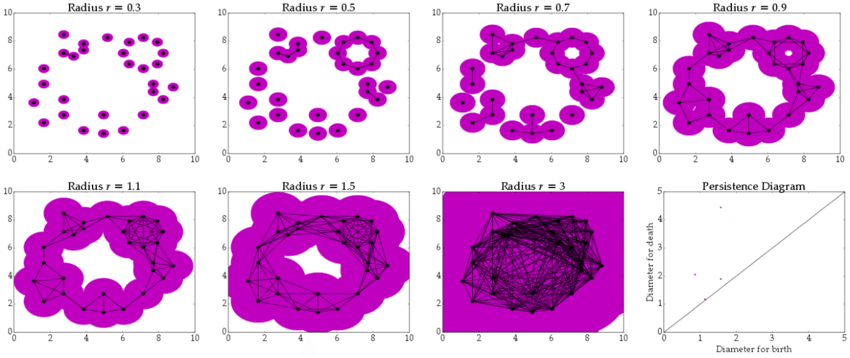
\includegraphics[scale=0.4]{./example.png}
        \source{Munch, Elizabeth. (2017). A User’s Guide to Topological Data Analysis. Journal of Learning Analytics. 4. 47-61. 10.18608/jla.2017.42.6. }
        \caption{An example of filtration}
    \end{figure}
\end{frame}

\begin{frame}{Persistent Homology}
    As simplicial complexes transform from one another, some simplicial complexes may appear (birth) and some others disappear (death). Persistence homology examines lifespan (\textcolor{myred}{persistence barcode}) of these.
    \begin{definition} 
        $H^{\delta,p}_k = Z^{\delta}_k/(B^{\delta+p}_k \cap Z^{\delta}_k)$ is called \textcolor{myred}{p-persistent $k^{th}$ homology} of $K^{\delta}$. \\
    \end{definition}
    Then, the corresponding Betti number is $\beta^{\delta,p}_k=rank(H^{\delta,p}_k)$. This is the number of $k$-dimensional holes that persist (neither birth nor death) during the interval $(\delta,\delta+p)$.
\end{frame}

\begin{frame}{Persistence Diagrams}
    For a simplicial complex, let $[s,t)$ represents its persistence barcode. Here $\delta=s$ is the birth and $\delta=t$ is the death. Then, each point $(s,t)$  has a \textcolor{myred}{multiplicity $\mu_{n}^{s,t}$} which is the number of simplicial comlexes that are born exactly at $s$ and die exactly at $t$. Then,
    \begin{align*}
        \mu_{n}^{s,t}=(\beta_{n}^{s,t-1}-\beta_{n}^{s,t})-(\beta_{n}^{s-1,t-1}-\beta_{n}^{s-1,t}).
    \end{align*}
    \textcolor{myred}{Persistence diagram} is the set of points (s,t), with multiplicities $\mu_{n}^{s,t}$ such that $0 \leq s < t \leq m+1$ where $m$ is the largest value of $\delta$.
\end{frame}

\begin{frame}{Persistence Diagrams (Example)}
    \begin{figure}
        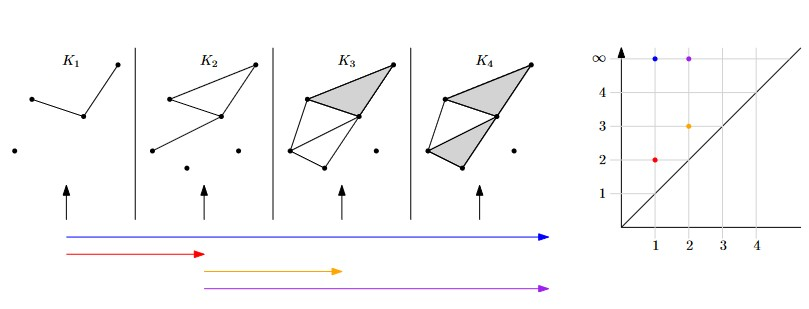
\includegraphics[scale=0.55]{./diagram.jpg}
        \source{Ž. Virk. Introduction to Persistent Homology. Založba UL FRI, University of Ljubljana, 2022, doi: 10.51939/0002. }
        \caption{Persistence barcodes and persistence diagram}
    \end{figure}
\end{frame}

\begin{frame}{Fundamental Lemma of Persistent Homology}
    \begin{lemma}[Fundamental Lemma of Persistence Homology] 
        Let $K^0 \subseteq K^1 \subseteq ... \subseteq K^m$ be a filtration. For every pair of indices $k,l$ such that $0 \leq k \leq l\leq m$, 
        \begin{align*}
            \beta_{n}^{k,l} = \sum\limits_{\substack{l < j, \\0 \leq i \leq k}}\mu_{n}^{i,j}
        \end{align*}
    \end{lemma}
    This equation implies that the information given by persistent Betti numbers are the same as the information given by barcodes or persistence diagrams.\cite{virk}
\end{frame}

\section{References}
\begin{frame}{References}
    \printbibliography
\end{frame}  
\end{document}